\chapter{Basics of Plotting}
\label{chp:plotting_functions}

\section{Plotting a Single Function}
\label{sec:plotting_a_single_function}

You can plot a function in Maple by using the \texttt{plot()} command. The only required parameter is the function you wish to plot. However, there are many additional parameters you can add to customise the way that the graph looks.

\marginnote{By default, Maple will plot trigonometric functions with an $x$-axis from $-2\pi$ to $2\pi$.}

\begin{maplegroup}
\begin{mapleinput}
\mapleinline{active}{1d}{plot(sin(cos(x)));
}{}
\index{plot}
\end{mapleinput}
\mapleresult
\mapleplot{tutorials/figures/Plotting_Functionsplot2d1a-eps-converted-to.pdf}
\end{maplegroup}

It is often useful to specify the interval for the $x$-axis. Choose left and right endpoint for the $x$-axis that are appropriate for your graph.\index{plot!axes intervals}

\marginnote{If you are plotting a function of $t$, then make sure to specify the interval as \texttt{t=a..b}.}

\begin{maplegroup}
\begin{mapleinput}
\mapleinline{active}{1d}{plot(sin(cos(x)), x=-10..10);
}{}
\end{mapleinput}
\mapleresult
\mapleplot{tutorials/figures/Plotting_Functionsplot2d1b-eps-converted-to.pdf}
\end{maplegroup}

\marginnote[1cm]{The order of the parameters in the \texttt{plot()} command is important. The interval for the $x$-axis must be listed before the interval for the $y$-axis.}
You can also specify the interval for the $y$-axis for your graph.\index{plot!axes intervals}

\begin{maplegroup}
\begin{mapleinput}
\mapleinline{active}{1d}{plot(sin(cos(x)), x=-10..10, y=-5..5);\index{plot!axes intervals}
}{}
\end{mapleinput}
\mapleresult
\mapleplot{tutorials/figures/Plotting_Functionsplot2d1c-eps-converted-to.pdf}
\end{maplegroup}

\section{Common Plot Options}
\label{sec:common_plot_options}

Table \ref{tbl:plot_options} lists the most frequently used optional parameters.

\begin{table}
\label{tbl:plot_options}
\centering
\begin{tabular}{lp{2.5in}}
\hline
Parameter & Description\\
\hline
\texttt{x=a..b}						& Plot over the interval $x\in[a,b]$.
    \index{plot!axes intervals}
    \\
\texttt{y=c..d}						& Plot over the interval $y\in[c,d]$.
    \index{plot!axes intervals}
    \\
\texttt{colour=}\textit{cname}		& Specify the colour of the graph.
    \index{plot!colours}
    \\
\texttt{discont=true}				& Show discontinuities in a function.
    \index{plot!axes intervals}
    \index{plot!discontinuities}
    \\
\texttt{linestyle=}\textit{lstyle}	& Specify the style of the line (\texttt{solid}, \texttt{dash}, \texttt{dot}, etc.).
    \index{plot!line style}
    \\
\texttt{gridlines=true}				& Include gridlines.
    \index{plot!gridlines}
    \\
\texttt{numpoints=}\textit{n}		& Set the minimum number of points plotted for a smoother graph (Default $200$).
    \index{plot!plot resolution}
    \\
\texttt{grid=[$m$,$n$]}				& Set the number of initial points used to plot a graph (Default $26 \times 26$).
    \index{plot!plot resolution}
    \\
\texttt{scaling=constrained}		& Force axes to use the same scale (so a circle should appear perfectly round).
    \index{plot!scaling}
    \\
\hline
\end{tabular}
\caption{A list of common optional parameters for the \texttt{plot()} command.}
\end{table}
\marginnote[-6cm]{A list of plot colours can be found by typing \texttt{?colours} on a new Maple input.}
\marginnote[-4cm]{Plotting commands often generate more than the minimum number of points. Setting \texttt{numpoints = 30000} may help if a graph does not appear smooth. Using too large of a value may cause Maple to become unresponsive (see Tutorial \ref{chp:implicit_functions}).}

The \texttt{discont=true} parameter may need to be included to properly display the discontinuities in certain functions when you plot them.

\begin{marginfigure}[-.1cm]
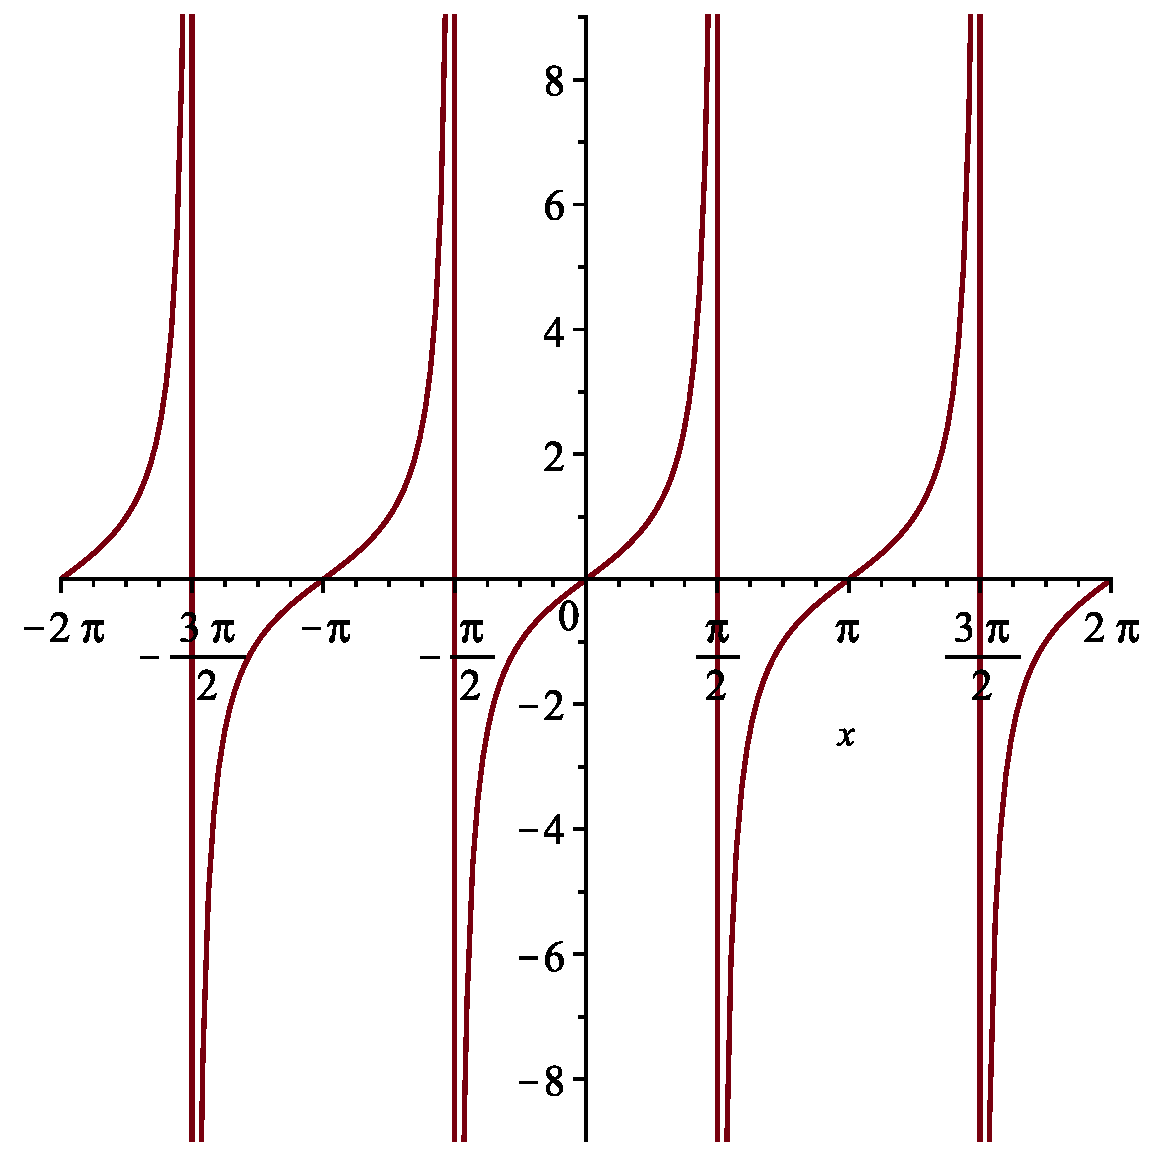
\includegraphics[width=5cm]{tutorials/figures/Plotting_Functionsplot2d2b-eps-converted-to.pdf}
\caption{Some versions of Maple may not correctly display the discontinuities in the graph of $\tan(x)$, as shown here. In this case, you need to include the \texttt{discont=true} parameter. Notice that the \texttt{linestyle=dashed} option was also excluded here.}
\end{marginfigure}

\begin{maplegroup}
\begin{mapleinput}
\mapleinline{active}{1d}{plot(tan(x), x=-2*Pi..2*Pi, y=-10..10, linestyle=dash, discont=true);
}{}
\end{mapleinput}
\mapleresult
\mapleplot{tutorials/figures/Plotting_Functionsplot2d3-eps-converted-to.pdf}
\end{maplegroup}
\begin{marginfigure}[-.8cm]
An example of a function that cannot be properly displayed without the \texttt{discont=true} parameter can be found on page \pageref{sec:limits_and_piecewise_functions}.
\end{marginfigure}
In some modern versions of Maple, the graph of $\tan(x)$ above can be obtained even without including the \texttt{discont=true} option in the \texttt{plot( )} command.

\section{Plotting Multiple Functions}
\label{sec:plotting_multiple_functions}

You can also plot multiple expressions and functions on the same graph using the \texttt{plot()} command. Instead of specifying a single function as your first parameter, create a list of functions using square brackets.

Similarly, instead of specifying a single colour, specify a list of colours using square brackets. The order of the functions matches the order of the colours.

\marginnote{If a list of colours is not specified when plotting multiple functions on the same graph, it may be difficult to match each curve to its corresponding function. The first three colours in Maple's default palette are dull shades of red, blue, and green.}
\begin{maplegroup}
\begin{mapleinput}
\mapleinline{active}{1d}{plot([exp(x), sin(x) + cos(x)], x=-10..10, y=-5..5, colour=[black, blue]);
}{}
\label{Plot!Plot multiple functions}
\end{mapleinput}
\mapleresult
\mapleplot{tutorials/figures/Plotting_Functionsplot2d2a-eps-converted-to.pdf}
\end{maplegroup}

If you need several complicated graphs to display at once, you may wish to explore the potential of the \texttt{display()} command, found in section \ref{sec:display_command} on page \pageref{sec:display_command}.